\documentclass[10pt]{beamer}

\usetheme{Warsaw}
%%%%%\usecolortheme{crane}
%%%%%\usecolortheme{orchid}
% \usecolortheme{orchid}
\definecolor{azull}{rgb}{.10,.20,.3}
\usecolortheme[named=azull]{structure}
\usefonttheme{structurebold}
%\usefonttheme{professionalfonts}
\useinnertheme{rounded}
\newcommand{\maggen}{\textbf{magGen}}
\usepackage[spanish]{babel}% division de silabas en spanish
\usepackage[utf8]{inputenc}
\usepackage{amsmath}
%\usepackage{amsfonts}
%\usepackage{amssymb}
%\usepackage{stmaryrd}
\usepackage{graphicx}
%\usepackage[all]{xy}
\usepackage{listings}
\definecolor{lbcolor}{rgb}{0.9,0.9,0.9}
\definecolor{gris}{rgb}{0.8,0.8,0.8}
\definecolor{azul}{rgb}{0.0,0.3,0.6}
\lstset{
    backgroundcolor=\color{lbcolor},
    tabsize=2,
    rulesepcolor=\color{azul},
    language=C++,
    morekeywords={repeat, until, procedure, then, from,
                  lexeme_d, as_lower_d, longest_d,
                  \!, \+, \*, \>\>, \-, \&, \|, \=, \%,
                  anychar_p, alnum_p, alpha_p, digit_p, lower_p, upper_p, space_p, ch_p, str_p, oct_p, hex_p, uint_p, int_p, real_p, eps_p, end_p,
                  symbols, add,
                  end},
    basicstyle=\tiny,
    aboveskip={1\baselineskip},
    columns=[c]fixed,
    showstringspaces=false,
    extendedchars=true,
    breaklines=true,
    prebreak = \raisebox{0ex}[0ex][0ex]{\ensuremath{\hookleftarrow}},
    frame=single,
    showtabs=false,
    showspaces=false,
    showstringspaces=false,
    identifierstyle=\ttfamily,
    keywordstyle=\color[rgb]{0.1,0.1,0.6}\bfseries,
    commentstyle=\color[rgb]{0.133,0.545,0.133},
    stringstyle=\color[rgb]{0.627,0.126,0.941},
    keepspaces=true,
    escapeinside=``,
    numbersep=5pt,
    numberstyle=\scriptsize
}

\lstdefinelanguage{specmag}{
  keywords={compute, end, all, semantic, domain, attributes, rules, sort, op, function, infix, prefix, postfix, syn, inh, left, right, non_assoc, and, and_eq, asm, auto, bitand, bitor, break, case, catch, class, compl, const, const_cast, continue, default, delete, do, double, dynamic_cast, else, enum, explicit, export, extern, false, for, friend, goto, if, inline, long, mutable, namespace, new, not, not_eq, operator, or, or_eq, private, protected, public, register, reinterpret_cast, return, short, signed, sizeof, static, static_cast, struct, switch, template, this, throw, true, try, typedef, typeid, typename, union, unsigned, using, virtual, void, volatile, wchar_t, while, xor, xor_eq, bool, char, float, int, string
%   ,repeat, until, procedure, then, from
  },
  sensitive=true,
  morecomment=[s]{/*}{*/},
  morecomment=[l]{\//},
  morestring=[d]{"}
}

\definecolor{linkcol}{rgb}{0,0,0.4} 
\definecolor{citecol}{rgb}{0.5,0,0} 
\setbeamercovered{transparent=5}

\subtitle[Generador de Evaluadores Estáticos para MAG]{Generador de Evaluadores Estáticos para MAG}
\title[Generador de Evaluadores Estáticos para MAG]{\maggen}
%\subtitle{Abstracci\'on: Acciones y Funciones}
\author{Gerardo Luis Kilmurray - Gonzalo Martín Picco}
\institute[U.N.R.C.]{
    Departamento de Computaci\'on\\
    Facultad de Ciencias Exactas, F\'isico-Qu\'imicas y Naturales\\
    Universidad Nacional de R\'io Cuarto}
% \date{Marzo de 2010}

\begin{document}

\frame{\titlepage}

\frame{
    \frametitle{Temario:}
    \tableofcontents
}

\section{\textquestiondown Qué es magGen?}

\frame{
\frametitle{\textquestiondown Qué es magGen?}
    \begin{block}{}
        \maggen\ es una herramienta generadora de evaluadores estáticos para la familia MAG. 
    \end{block}
    
    \begin{center}
        {\huge \textbf{mag} + \textbf{Gen}}\\
        \textit{Multi-plans Attribute Grammar} - \textit{Generator}
    \end{center}

    Características distinguibles:
    \begin{itemize}
        \item Basa su funcionamiento en gramática MAG.
        \item Generación de mínima cantidad de planes.
        \item Generación de Evaluadores estáticos.
    \end{itemize}
}

\subsection{Motivación}
\frame{
    \begin{block}{}
        En las ciencias de la computación los lenguajes juegan un rol muy importante en muchas disciplinas. Desde los comienzos se buscaron \textit{mecanismos} para describirlos y manejarlos.
    \end{block}
    
    \begin{block}{}
        Desde que D. Knuth introdujo en 1966 las \textbf{gramáticas de atributos} (GA), estas se han utilizado ampliamente para el desarrollo de herramientas de procesamiento de lenguajes formales, como compiladores, intérpretes, traductores, así  como también para especificar la semántica de lenguajes de programación.
    \end{block}
    
    \begin{block}{}
        En 1998, Wuu-Yang caracteriza una nueva familia denominada \textbf{Gramática de Atributos Multi-planes}. 
    \end{block}
    
    \begin{center}
        \textbf{Al momento no existían herramientas basadas en esta familia de Gramáticas de Atributos}
    \end{center} 
}

\section{Preliminares}

\frame{
    \frametitle{Notación}
    \begin{block}{Gramatica de atributos (Informal)}
        En una \textbf{Gramática de Atributos} (GA), se relaciona cada símbolo de una \textit{Gramática Libre de Contexto} con un conjunto de atributos. Cada regla o producción tiene asociado un \textit{conjunto de reglas semánticas}, denominadas también \textit{ecuaciones}.
    \end{block}

    \textbf{Instancia:} Ocurrencia de un símbolo de la gramatica asociado a un atributo. 
}

\begin{frame}[fragile]
    \frametitle{Ejemplo GA}

    \begin{lstlisting}
         (R1)   S `$\rightarrow$` XYZ      
                  S.s0 := X.s1 + Y.s2 + Y.s3 + Z.s4
                  X.i1 := Y.s3  
                  Y.i2 := X.s1
                  Y.i3 := Y.s2
         (R2)   Y `$\rightarrow$` m        
                  Y.s2 := Y.i2
                  Y.s3 := 1
         (R3)   Y `$\rightarrow$` n        
                  Y.s2 := 2
                  Y.s3 := Y.i3
         (R4)   X `$\rightarrow$` m        
                  X.s1 := X.i1
         (R5)   Z `$\rightarrow$` Y        
                  Z.s4 := Y.s3
                  Y.i2 := 3
                  Y.i3 := Y.s2
    \end{lstlisting} 

    \begin{block}{Ejemplo instancia}
        Y.i3 $\Leftrightarrow$ Ocurrencia del simbolo $Y$ asociado al atributo $i3$.
    \end{block}
\end{frame}

\subsection{Familia de Gramáticas de Atributos Multiplanes (MAG)}

\frame{
    \frametitle{Gramáticas de Atributos Multiplanes}

	\begin{block}{Dependencias directas de una producción}
        Se denota como \textbf{DP(p)}	
        $$
          DP(p) = \{(X_{i}.a, X_{j}.b) | X_{i}.a \rightarrow Y_{j}.b \in R^{p} \}
        $$
    \end{block}
    
    Dado un símbolo X de una gramática de atributos

    $$\textbf{Down(X)} =  \{(a,b) | a \rightarrow b \} con\ a,b \in A(X)\}$$
}

\frame{
    \frametitle{Gramáticas de Atributos Multiplanes (cont.)}

    \begin{block}{Conjunto de dependencias aumentadas}
        Sea $q$ una producción de la forma $X_{0}\rightarrow \alpha_{0} X_{1} \alpha_{1} X_{2} \dots X_{k} \alpha_{k}$. Sea $p_{i}$ una producción cuya parte izquierda es $X_{i}$ ($1\leqslant i \leqslant k$). 
        $$
        ADP (q | p_{1}, p_{2}, \dots, p_{k}) = DP(q) \bigcup\limits_{k}^{i=1}{DGC_{X_{i}}} (p_{i})
        $$
        se denota como $\textbf{ADP (q $|$ p}_{\textbf{1}}\textbf{, p}_{\textbf{2}}\textbf{, \dots , p}_{\textbf{k}}\textbf{)} $
    \end{block}
    
    $\textbf{DCG}_{\textbf{X}}\textbf{(p)}$ contiene las dependencias, entre las instancias de la gramática, para el símbolo \texttt{X}, acotando el análisis para la producción \textit{p} y los posibles contextos inferiores.
    $$
    \bigcup\limits_{\textit{todo p}}{DCG_{X} (p) = Down (X)}
    $$
}

\frame{
    \frametitle{Gramáticas de Atributos Multiplanes (cont.)}
    El conjunto de todas las posibles dependencias aumentadas para una producción q se define como:
    $$
    SADP(q) = \bigcup\limits_{q\in P}{ADP (q | p_{1}, p_{2}, \dots, p_{k})} 
    $$

    \begin{block}{Gramatica de atributos Multiplanes}
        Una gramática \textit{G} es una \textit{gramática de atributos multi-planes} si y solo si 
        $$
        \forall q : q \in P: (\forall g:g\ es\ un\ grafo\ de\ q \wedge g \in SADP(q) : g\ es\ no\ circular) 
        $$
    \end{block}
}

\subsection{Evaluador estático}

\frame{
    \frametitle{Evaluador estático}
    
	\begin{block}{}
    	Los métodos estáticos deben tener en cuenta todos los árboles sintácticos posibles a ser generados por la gramática y calcular las dependencias, entre las instancias de los atributos, para cada uno de ellos. 
	\end{block}

    \begin{block}{Contexto de una producción}
        Dada una producción $p$ se deben tener en cuenta tres tipos de dependencias que definen el \textit{contexto} de la misma:

        \begin{itemize}
            \item Directas obtenidas por las ecuaciones de $p$.
            \item Impuestas por el contexto superior.
            \item Impuestas en el contexto inferior.
        \end{itemize}
    \end{block}

    Instancias diferentes de una producción $p$ tendrán las mismas dependencias directas, pero podrán tener diferentes dependencias impuestas por los contextos inferiores y superiores. 
}

\subsection{Planes de evaluación}

\frame{
    \frametitle{Planes de evaluación}

    \begin{block}{}
        Luego del análisis de las dependencias, se conocen que ecuaciones tienen que computarse antes que otras.
    \end{block}

    \begin{block}{}
        Este proceso se realizó sobre las estructuras abstractas de la gramática, así que los resultados obtenidos se aplican a \textbf{todas} las cadenas que se pueden producir, más concretamente, a todos los AST válidos en la gramática.
    \end{block}

	\begin{block}{Plan de Evaluación}
    	Un plan de evaluación esta dado por un orden consistente con las dependencias para la computación de las ecuaciones que definen a cada instancia de la gramatica.
	\end{block}
}

\subsection{Secuencias de visitas}
\frame{
	\frametitle{Secuencia de Visita}
	
	\begin{block}{}
	El concepto de \emph{Secuencias de Visita} fue presentado en 1980, por \textbf{Uwe Kastens}  como un método de evaluación para la familia $OAG$.
	\end{block}
	
	Basa su funcionamientos en la visita de los nodos de los arboles de derivacion para lograr la evaluacion del arbol. Este metodo se apoya en los planes de evaluacion de la gramatica.
}

\frame{
    \frametitle{Secuancia de Visita (cont)}

	\begin{block}{Definición}
    	Sea $n$ un nodo de un árbol atribuido $T$. Una secuencia de visita en el nodo $n$ \textbf{es una secuencia de tres operaciones o acciones}: 
    	\emph{visit(child,i)}, \emph{compute(at)} y \emph{leave(i)}.
    \end{block}

	\begin{description}
    	\item [visit(child,i)] indica que el evaluador debe moverse (visitar) el nodo hijo \emph{child} de $n$ y corresponde a la \emph{i-ésima} visita al nodo hijo.

    	\item [compute(at)] indica que debe evaluarse la ecuación que define $at$ en la producción $p$ aplicada correspondiente al nodo $n$.

    	\item[leave(i)] indica que ha finalizado la visita \emph{i-ésima} en el nodo corriente y que se debe visitar al nodo padre.
	\end{description}
}

\section{maggen}

\subsection{Diseño}

\frame{
    \frametitle{\maggen: Funcionamiento}
    
    El funcionamiento de \maggen\ esta dado por la integración de 4 etapas, consideradas principales, que marcaron el proceso de desarrollo de la herramienta:
    \begin{itemize}
        \item Lenguaje especificación de MAG.
        \item Parser del lenguaje,representación interna y chequeos.
        \item Construcción de grafos y aplicación de algoritmos de cómputo de planes y secuencias de visita.
        \item Generación de código.
    \end{itemize}

    El cómputo de \maggen\ se realiza atravesando cada una de estas etapas secuencialmente, es decir, la terminación exitosa de una, habilita la siguiente; por lo tanto cada etapa mantiene su salida de errores de manera independiente. 
}

\begin{frame}[fragile]
    \frametitle{\maggen: Funcionamiento (cont.)}

    La salida normal de \maggen\ que indica que se han realizado todas las etapas correctamente, es la siguiente:

%    \vspace{0.3cm}
    \begin{lstlisting}[backgroundcolor=\color{white}, basicstyle=\scriptsize, language=]
        * Parsing grammar ---------- [  OK  ]
        * Generate graphs ---------- [  OK  ]
        * Build plans -------------- [  OK  ]
        * Build visit sequence ----- [  OK  ]
        * Generation code ---------- [  OK  ]

        Generation complete in: 0.372814 seconds.
    \end{lstlisting}
%    \vspace{0.3cm}
\end{frame}

\frame{
    \frametitle{Tesis}

    \begin{block}{Tema seleccionado}
        Gram\'aticas de Atributos con Multiplanes de Evaluaci\'on (MAG)
        \footnote{WUU YANG. - http://www.cis.nctu.edu.tw/~wuuyang/./papers/magAPSEC.ps}.
    \end{block}
    \pause

    \begin{exampleblock}{Objetivo Espec\'ifico}
        \begin{center}
            \textbf{\\Generador de Evaluadores Est\'aticos de MAG.}
            \vspace{0.3cm}
        \end{center}
    \end{exampleblock}
}

\frame{
    \frametitle{magGen: Herramientas usadas}

    \begin{tabular}{p{4.5cm}p{6.5cm}}
    \begin{itemize}
	    \item C++%\footnote{http://public.research.att.com/~bs/C++.html}.
		\item Boost C++ Libraries%\footnote{http://www.boost.org/}.
		    \begin{itemize}
			\item Spirit Parser Framework%\footnote{http://boost-spirit.com/home/}.
			\item The Boost Graph Library (BGL)%\footnote{http://www.boost.org/doc/libs/release/libs/graph/}.
		    \end{itemize}
		\item GraphViz% \footnote{http://www.graphviz.org/}.
        \item Eclipse 
		\item Subversion 
		\item \LaTeXe 
	\end{itemize}&
	\begin{itemize}
		\item kile 
		\item Graphviz 
		\item Nemiver 
		\item Dia 
		\item Bouml 
		\item Cmake 
		\item Análisis estático de código:
		\begin{itemize}
			\item CCCC 
			\item gcov 
		\end{itemize}
	\end{itemize}\\
	\end{tabular}
}

\frame{
    \frametitle{magGen}

    \begin{block}{Proceso de generaci\'on}
	    \begin{itemize}
    		\item Parsing de la MAG.
    		\pause
    		\item Generaci\'on de estructuras internas.
    		\pause
    		\item Verificaci\'on de propiedades inherentes a gram\'aticas.
    		\pause
    		\item Generaci\'on de grafos de DP, Down, DCG y ADP para cada regla y s\'imbolo.
    		\pause
    		\item Comprobaci\'on de ciclicidad sobre cada tipo de grafo.
    		\pause
    		\item Generaci\'on de Planes de Evaluaci\'on.
    		\pause
    		\item Generaci\'on de Secuencias de Visitas.
    		\pause
    		\item Generaci\'on de c\'odigo fuente del evaluador.
	    \end{itemize}
    \end{block}
}

\begin{frame}[fragile]
    \frametitle{magGen}

    \begin{block}{Informaci\'on de input del generador}
        Especificaci\'on de una MAG:
    \end{block}
        
    \begin{lstlisting}[language=specmag, basicstyle=\small]
        semantic domain
            <sorts>
            <operators>
            <functions>
        attributes
            <attrs>
        rules
            <r0>
                <eqs>
            `$\ldots$`
            <rN>
                <eqs>
    \end{lstlisting} 

\end{frame}

\frame{
        \frametitle{magGen - Grafo DP}
	    \begin{center}
% 		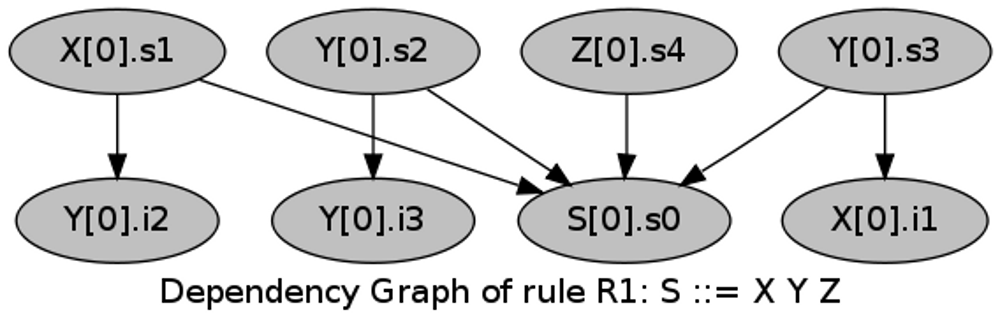
\includegraphics[scale=0.5]{./1_dp_graph.png}
		% 1_dp_graph.png: 568x188 pixel, 72dpi, 20.04x6.63 cm, bb=0 0 568 188
	    \end{center}
}

\frame{
        \frametitle{magGen - Grafo Down}
	    \begin{center}
% 		\includegraphics[scale=0.6]{./6_down_graph.png}
		% 6_down_graph.png: 176x92 pixel, 72dpi, 6.21x3.25 cm, bb=0 0 176 92
	    \end{center}
}

\frame{
        \frametitle{magGen - Grafo DCG}
	    \begin{center}
% 		\includegraphics[scale=0.5]{./10_dcg_graph.png}
		% 10_dcg_graph.png: 485x92 pixel, 72dpi, 17.11x3.25 cm, bb=0 0 485 92
	    \end{center}
}

\frame{
        \frametitle{magGen - Grafo ADP}
	    \begin{center}
% 		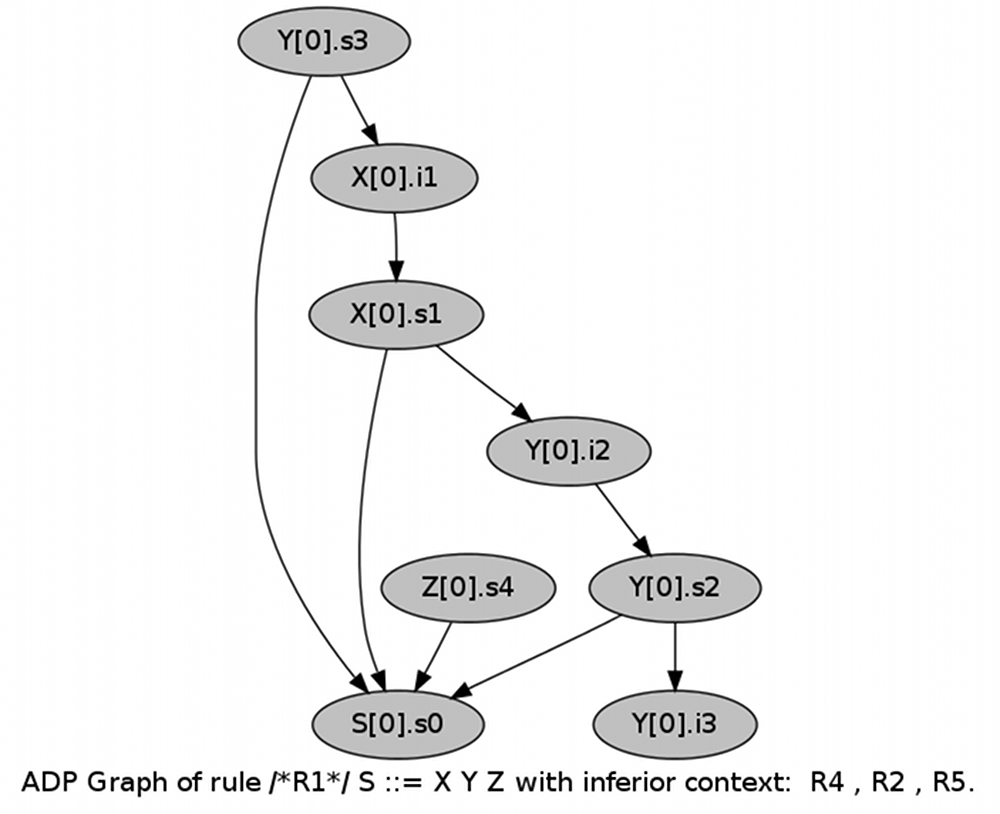
\includegraphics[scale=0.35]{./15_adp_graph.png}
		% 15_adp_graph.png: 676x572 pixel, 72dpi, 23.85x20.18 cm, bb=0 0 676 572
	    \end{center}
}

\frame{
        \frametitle{magGen - Grafo ADP}
	    \begin{center}
% 		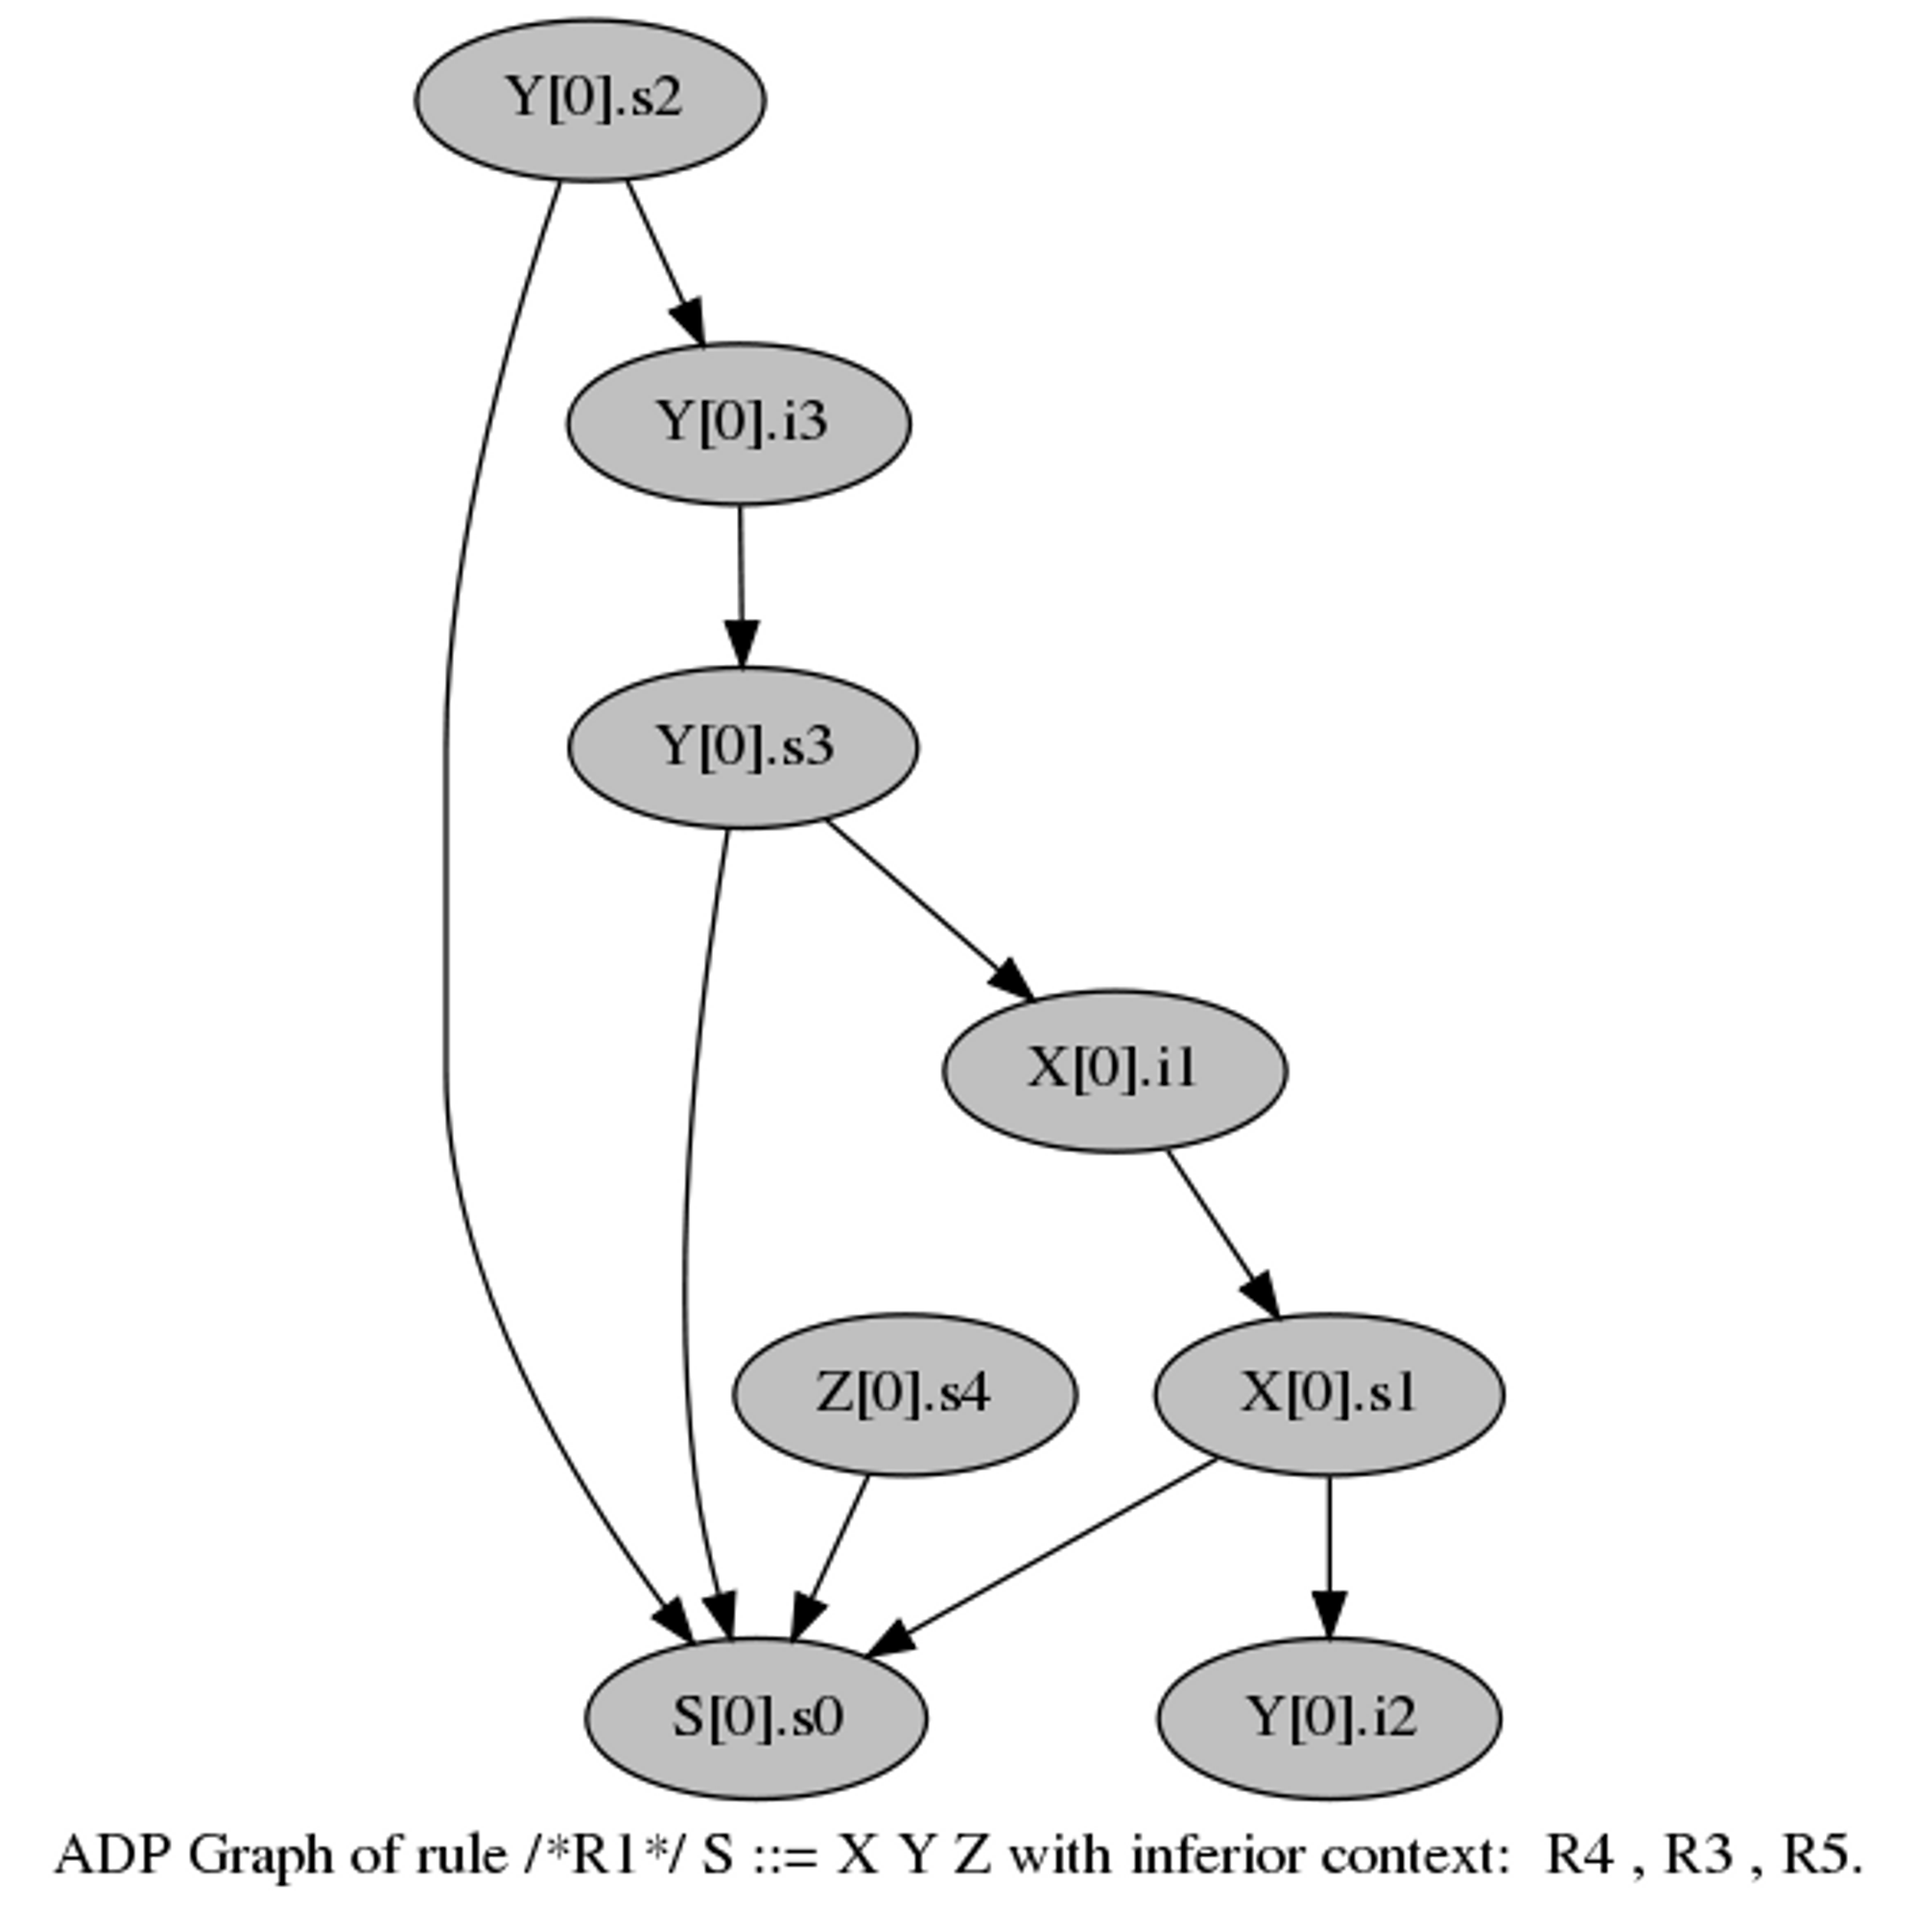
\includegraphics[scale=0.35]{./16_adp_graph.png}
		% 16_adp_graph.png: 676x572 pixel, 72dpi, 23.85x20.18 cm, bb=0 0 676 572
	    \end{center}
}

\frame{
        \frametitle{magGen - Plan de evaluaci\'on}
	    \begin{center}
% 		\includegraphics[scale=0.32]{./22_plan_graph.png}
		% 22_plan_graph.png: 987x380 pixel, 72dpi, 34.82x13.41 cm, bb=0 0 987 380
	    \end{center}
}

\frame{
        \frametitle{magGen - Plan de evaluaci\'on}
            \begin{center}
% 		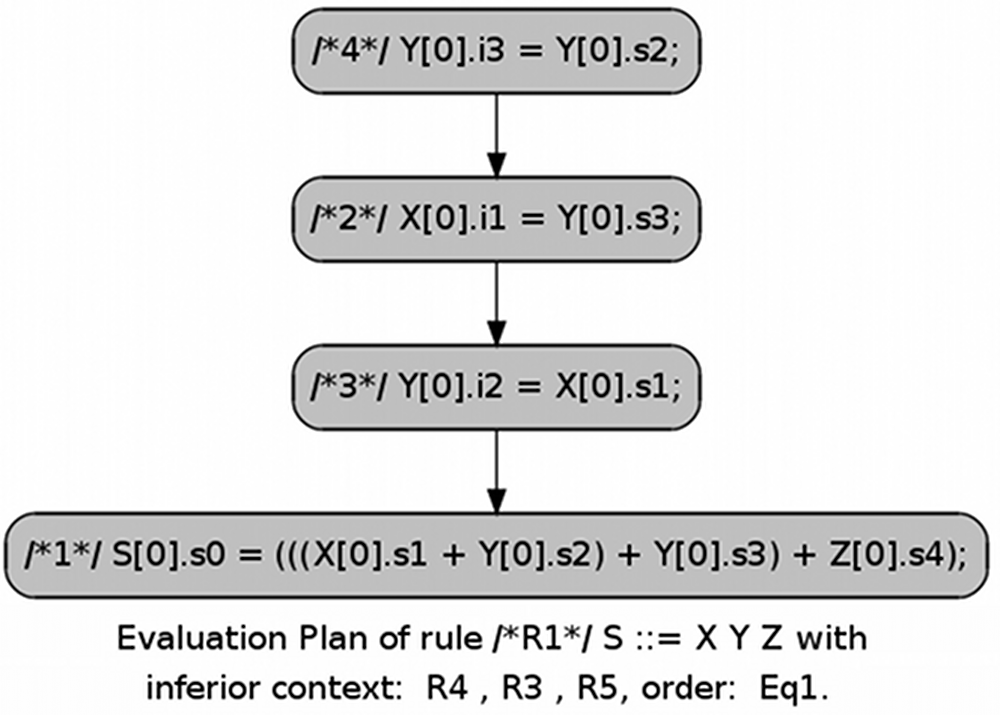
\includegraphics[scale=0.32]{./23_plan_graph.png}
		% 23_plan_graph.png: 987x380 pixel, 72dpi, 34.82x13.41 cm, bb=0 0 987 380
	    \end{center}
}

\frame{
        \frametitle{magGen - Secuencia de visita}
	
        \begin{block}{Secuencia de visita generada para el plan\\ R1 $\rightarrow$ R2 R3 R4}
	    \begin{center}
		\vspace{0.1cm}
		\textbf{Visit R2 $\Rightarrow$\\
			\vspace{0.1cm}
			Compute X[0].i1 $\Rightarrow$\\
			\vspace{0.1cm}
			Visit R4 $\Rightarrow$\\
			\vspace{0.1cm}
			Compute Y[0].i2 $\Rightarrow$\\
			\vspace{0.1cm}
			Visit R2 $\Rightarrow$\\
			\vspace{0.1cm}
			Compute Y[0].i3 $\Rightarrow$\\
			\vspace{0.1cm}
			Visit R5 $\Rightarrow$\\
			\vspace{0.1cm}
			Compute S[0].s1} 
	    \end{center}
	\end{block}
}

\frame{
        \frametitle{magGen}

        \begin{block}{Informaci\'on de input del evaluador}
            \'Arboles Atribu\'idos representados con AST\footnote{Attribute Syntax Tree}.
        \end{block}
        \pause

        \begin{block}{Informaci\'on de output del evaluador}
            El AST decorado\footnote{Cada uno de sus atributos se encuentran calculados}.
        \end{block}
}

\frame{
        \frametitle{magGen}

        \begin{block}{Objetivo Subyacente}
            Implementar Lenguages de Prop\'ositos Espec\'ificos para problemas puntuales.
        \end{block}
}

\subsection{Detalles de implementación}
\frame {
	\begin{block}{}
		bla bla
	\end{block}
}


\subsection{Evaluador generado}
\frame {
	\begin{block}{}
		bla bla
	\end{block}
}


\section{Comentarios Finales}
\frame {
	\begin{block}{}
		bla bla
	\end{block}
}

\section{Bibliografía}
   \begin{frame}
   \small{Bibliografía} 
   \begin{thebibliography}{66}
    \scriptsize{
    \bibitem{1} \textbf{\textit{``Calculo de Programas''}}\\  - J. Blanco, S. Smith y Damián Barsotti.
    \bibitem{2} \textbf{\textit{``An axiomatic basis for computer programming''}}\\ - Charles Antony Richard Hoare.
    \bibitem{3} \textbf{\textit{``Guarded commands, nondeterminacy and formal derivation of program''}}\\ - Edsger W. Dijkstra
    \bibitem{3} \textbf{\textit{``Assigning meanings to programs''}}\\ - Robert W. Floyd.
    \bibitem{4} \textbf{\textit{``Communicating sequential processes''}}\\  - Charles Antony Richard Hoare.
    \bibitem{5} www.wikipedia.org
    }
    \end{thebibliography}
    \end{frame}

\end{document}
